% Research articles should be limited to 15,000 words, including references and figure captions.
% run `biber manuscript` in terminal before knitting after adding any new refs

\documentclass{article}
\usepackage[utf8]{inputenc}
\usepackage{authblk}
\usepackage{setspace}
\usepackage[margin=1.25in]{geometry}
\usepackage{graphicx}
\graphicspath{ {../figures/} }
\usepackage{subcaption}
\usepackage{amsmath}
\usepackage{lineno}
\linenumbers
\usepackage[T1]{fontenc} % to avoid issues with special fonts in bib file
\usepackage{xcolor} % for colored draft text
\usepackage{hyperref}

%%%%%% Bibliography %%%%%%
% Replace "sample" in the \addbibresource line below with the name of your .bib file.
\usepackage[style=nejm,
citestyle=numeric-comp,
sorting=none]{biblatex}
% \usepackage[style=remote-sensing-of-environment]{biblatex}
\addbibresource{ndvi-stochasticity.bib}

%%%%%% Title %%%%%%
% Full titles can be a maximum of 100 characters, including spaces. 
% Title Format: Use title case, capitalizing the first letter of each word, except for certain small words, such as articles and short prepositions
\title{DENVar: A Global Dynamic Estimate of NDVI Variance}

%%%%%% Authors %%%%%%
% Authors should be listed in order of contribution to the paper, by first name, then middle initial (if any), followed by last name.
% Authors should be listed in the order in which they will appear in the published version if the manuscript is accepted. 
% Use an asterisk (*) to identify the corresponding author, and be sure to include that person’s e-mail address. Use symbols (in this order: †, ‡, §, ||, ¶, #, ††, ‡‡, etc.) for author notes, such as present addresses, “These authors contributed equally to this work” notations, and similar information.
% You can include group authors, but please include a list of the actual authors (the group members) in the Supplementary Materials.
\author[1,2]{Stefano Mezzini}
\author[3]{Gavin L Simpson}
\author[1,2,4,*]{Michael J Noonan}

%%%%%% Affiliations %%%%%%
\affil[1]{Okanagan Institute for Biodiversity, Resilience, and Ecosystem Services, The University of British Columbia Okanagan, Kelowna, British Columbia, Canada.}
\affil[2]{Department of Biology, The University of British Columbia Okanagan, Kelowna, British Columbia, Canada.}
\affil[3]{Department of Animal and Veterinary Sciences, Aarhus University, Denmark.}
\affil[4]{Department of Computer Science, Math, Physics, and Statistics, The University of British Columbia Okanagan, Kelowna, British Columbia, Canada.}
\affil[*]{Address correspondence to: michael.noonan@ubc.ca}

%%%%%% Date %%%%%%
% Date is optional
\date{}

%%%%%% Spacing %%%%%%
% Use paragraph spacing of 1.5 or 2 (for double spacing, use command \doublespacing)
\onehalfspacing

\begin{document}

% references from appendices that may not appear in the main text
\nocite{crameri_geodynamic_2018, crameri_scientific_2018, okabe_color_2008, frerebeau_khroma_2024, olson_terrestrial_2001}

\maketitle

%%%%%% Abstract %%%%%%
\begin{abstract}
Remote-sensing proxies of habitat productivity such as the Normalized Difference Vegetation Index (NDVI) have helped develop and support many hypotheses and projects. However, historically, users tended to focus solely on trends in mean productivity. In recent years, the variance around the mean (i.e., stochasticity) has gained more attention, particularly as climate change and human-induced rapid environmental change transform the ecosystems species have evolved in and adapted to. Still, calculating trends in NDVI stochasticity requires careful modeling, since stochasticity estimates are conditional on the estimated mean and the scale at which the data are collected and modeled. We thus present a new global Dynamic Estimate of NDVI Variance, \emph{DENVar}. We estimate spatiotemporal trends in NDVI mean and variance using Generalized Additive Models, which provide a flexible yet transparent and interpretable model structure. We show that DENVar correlates nonlinearly with \emph{\textbf{XXX}} and can be used to test many hepotheses related to environmental stochasitcity, such as optimal foraging theory and regime shifts as well as for conservation. We provide a publicly and freely available repository for downloading rasters of daily and long-term averages of DENVar and the related estimates of mean NDVI.
\end{abstract}

\clearpage

%%%%%% Main Text %%%%%%

\section{Introduction}

The Normalized Difference Vegetation Index (NDVI) is a proxy of primary productivity used in a wide range of disciplines, including ecology \cite{pettorelli_using_2005, pettorelli_normalized_2011}, landscape phenology \cite{merkle_large_2016, hmimina_evaluation_2013}, agriculture \cite{franch_30_2017}, forestry \cite{joao_indicator-based_2018}, and conservation \cite{mallegowda_assessing_2015, marcus_planning_2025}. High-resolution, remotely-sensed NDVI data have allowed analysts to estimate plant biomass without fieldwork \cite{bhatti_field_2024, borowik_normalized_2013} and leverage such estimates for studying large-scale plant dynamics \cite{pettorelli_using_2005} and their effects on animal movement behavior \cite{merkle_large_2016, aikens_greenscape_2017}. Still, most NDVI work is limited to quantifying changes in and responses to mean NDVI while ignoring changes in the variance around the mean.

Environmental stochasticity has been studied for decades \cite{levins_evolution_1974, stephens_optimal_1982, lande_risks_1993, saether_environmental_1997}, but recent work has drawn more attention to the effects environmental stochasticity has at a wide range of scales, from individual organisms \cite{mezzini_how_2025, rizzuto_forage_2021} to landscapes \cite{zhang_ndvi_2009, mutti_ndvi_2020, marcus_planning_2025}. However, estimating trends in NDVI variance requires more nuanced modeling than estimating changes in mean NDVI, particularly when environments are temporally dynamic and spatially heterogeneous. The scale at which processes are observed determine how individuals' perception of and ability to respond to change \cite{levin_problem_1992}. A forest fire is severely disruptive and deadly for many insects \cite{fettig_fire_2022}, while birds and large mammal may not struggle to escape the fire and or establish a new range \cite{franklin_relative_2021, calhoun_movement_2024}. Similarly, the effects of the fire recovery will depend on its duration relative to other organisms' phenology and lifespan \cite{frankham_importance_2004}. Therefore, distinguishing between a change in mean NDVI and a stochastic fluctuation requires a conscious decision about the scale at which to consider the data.

Previous work suggests that environmental stochasticity can reduce limit species' ability to adapt or specialize \cite{chevin_adaptation_2010}, alter species' movement behavior \cite{mezzini_how_2025}, and even affect extinction risk at both the population and species levels \cite{lande_risks_1993, bull_metapopulation_2007, fung_quantifying_2018}. Still, the effects of environmental stochasticity on species dynamics and ecosystem stability remain understudied \cite{marcus_changing_2023}. Global, temporally dynamic estimates of NDVI variance would facilitate research by building upon the widespread use and interpretability of NDVI wile also removing the barriers of computational demand and statistical knowledge that are required for quantifying environmental stochasticity. However, since NDVI is not a direct measurement primary productivity but a proxy, it should be interpreted carefully \cite{pettorelli_normalized_2011}. NDVI is prone to sensitivity loss in very green environments \cite{matsushita_sensitivity_2007, son_comparative_2014}, values vary across sensors \cite{beck_global_2011, fan_global_2016, huang_commentary_2021}, and the coarse spatiotemporal scale of satellite-derived NDVI can be a substantial barrier when assessing fine-scale trends \cite{goodchild_scale_2023, reid_its_2018}. However, careful statistical modeling can help overcome some of these limitations. In particular, Generalized Additive Models (GAMs) are particulalrly convenient due to their ability to learn flexibly from data \cite{wood_generalized_2017, simpson_modelling_2018} and handle very large spatiotemporal datasets \cite{wood_generalized_2015, wood_generalized_2017-1}.

We present a new measure of environmental stochasticity, which we name the Dynamic Estimate of NDVI Variance (DENVar). We calculate DENVar using 44 years of NDVI data from the AVHRR and VIIRS collection of sensors and GAMs. Although satellites with AVHRR and VIIRS sensors provide data at a coarser spatial resolution (0.05\textdegree) than other satellites (e.g., 250m for MODIS), they are the only sensors to provide data at a daily frequency and and for more than 40 years. Our use of GAMs provides a flexible yet interpretable approach for estimating trends in mean and variance in NDVI without the rigidity of other more traditional methods (e.g., ARIMA) or the opaqueness of machine learning models such as neural networks \cite{simpson_modelling_2018, wood_generalized_2017}. We illustrate the relationships between DENVar and multiple, relevant ecological metrics, and we provide access to a free repository of daily, global estimates of DENVar and the corresponding estimates of mean NDVI.

\section{Methods}

\subsection{Choice of color palettes}

We represent NDVI using a modified version of Fabio Crameri's divergent \emph{bukavu} palette \cite{crameri_geodynamic_2018, crameri_misuse_2020}, which has high-contrast for deuteranope and protanope vision. For NDVI values between -0.1 and 1, the colors also have sufficient contrast for the colors to also be distinguishable by strong tritanope and achomatic vision. Fig. A.1 contains an approximate representation of how each vision type would perceive each color palettes used. We obtained all color palettes with three or more colors from the \texttt{khroma} package (v. 1.14.0, \cite{frerebeau_khroma_2024}) for \texttt{R} (v. 4.4.0, \cite{r_core_team_r_2024}).

\subsection{Datasets used} \label{m-data}

\begin{figure}[h]
    \centering
    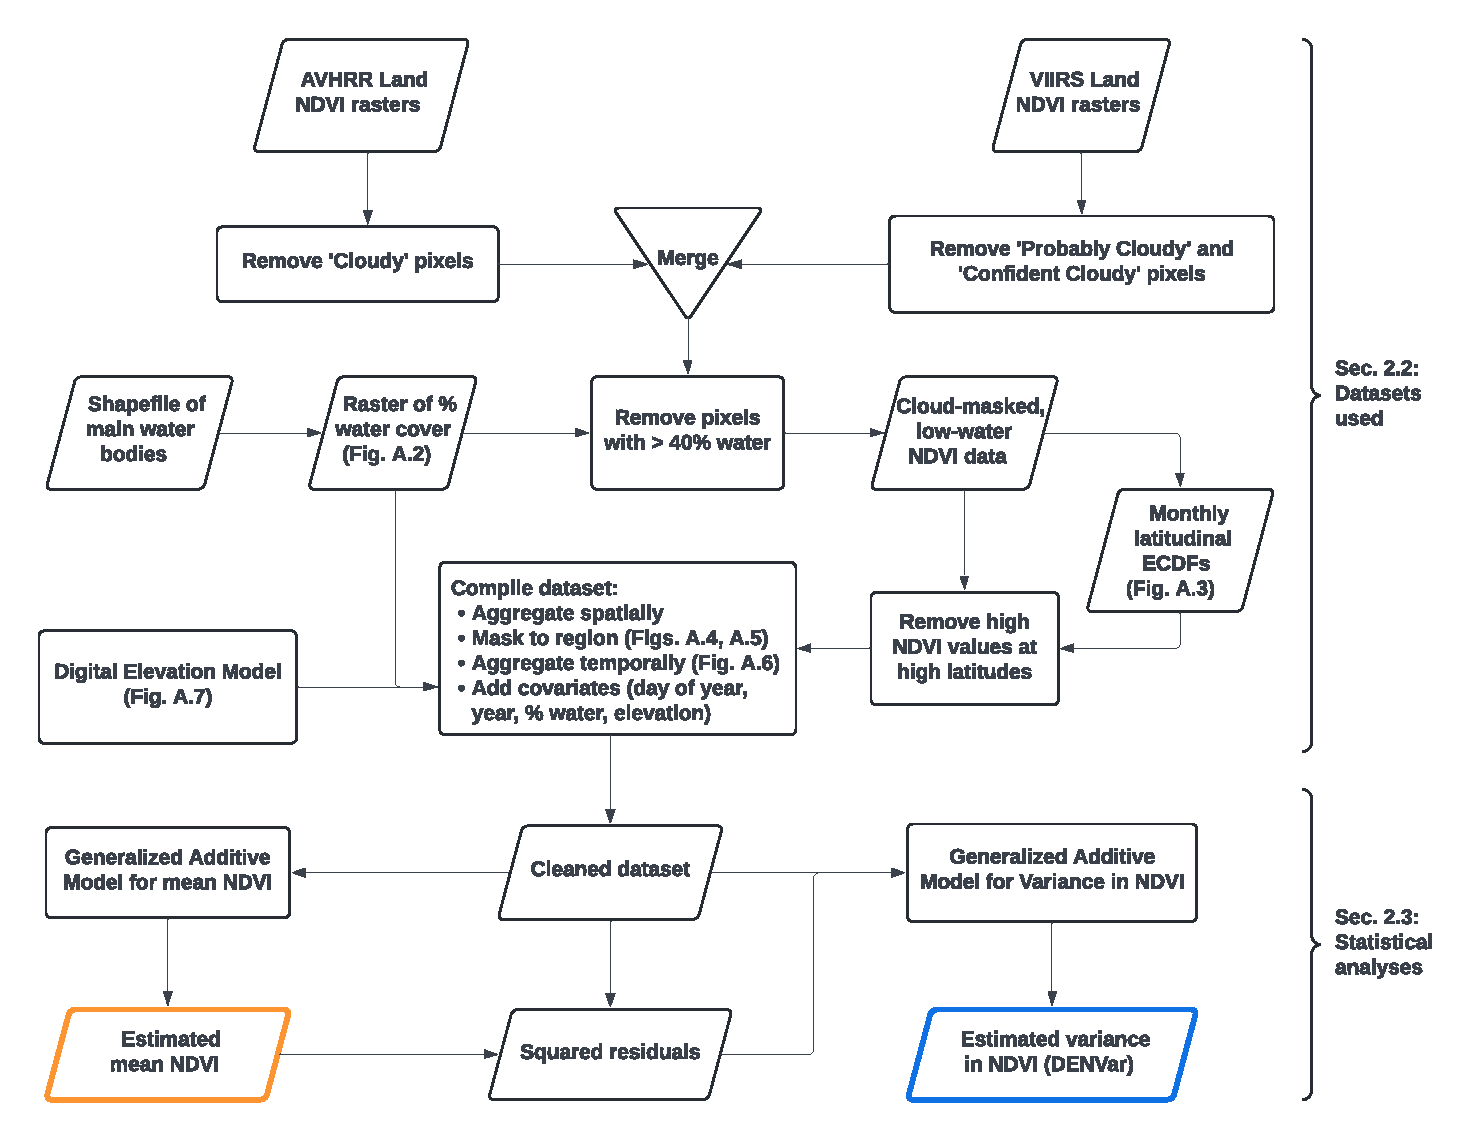
\includegraphics[width=\textwidth]{flowchart/denvar-flowchart}
    \caption{\textbf{Flowchart for the analyses used in the manuscript. The curly braces on the right indicate the subsections in the Methods section that detail the dataset collation and cleaning (\ref{m-data}.), and statistical analyses (\ref{m-analyses}).}
    \label{analysis-diagram}
\end{figure}

Fig. \ref{fig:analysis-diagram} illustrates the processes of data collection, cleaning, and modeling used in this project. We downloaded NDVI image composites directly from the servers for data from AVHRR sensors (1981-06-24 to 2013-12-31; \href{https://ladsweb.modaps.eosdis.nasa.gov/archive/allData}{https://ladsweb.modaps.eosdis.nasa.gov/archive/allData}; \cite{vermote_noaa_2018}) and VIIRS sensors (2014-01-01 to 2025-06-29; \href{https://ncei.noaa.gov/data}{https://ncei.noaa.gov/data/}; \cite{vermote_noaa_2022}).

We removed all pixels labeled as "cloudy" for AVHRR rasters and "probably cloudy" or "confidently cloudy" for VIIRS ratsers. To remove pixels that included large portions of water, we used a shapefile of major water bodies (\cite{garmin_international_inc_world_2025}) to produce a static raster of the percentage of water within each pixel, at the same spatial resolution as the NDVI rasters (0.05\textdegree; Fig. A.2). We removed all pixels with > 40\% water cover.

Many rasters had horizontal bands of NDVI > 0.9 at unrealistically northern latitudes between September and March, likely due to limited visibility during fall and winter in the Northen hemisphere. We identified and removed problematic pixels using the monthly empirical cumulative distribution functions of NDVI across latitude (Fig. A.3). We did not filter problematic values at latitudes $< 60^\circ$S since we fully excluded Antarctica from the analyses (Fig. A.4).

To ensure the number of rows for each dataset was below the maximum data frame size in \texttt{R} ($3.17 \times 10 ^{10} > 2^{31} - 1 \approx 0.21 \times 10^{10}$), we reduced the dataset size by splitting it across four spatial groups (Figs. A.4 and A.5) and spatially and temporally aggregated the rasters by a factor of four. The final dataset thus had one raster every four days with a spatial resolution of $0.05^\circ\times4=0.2^\circ$ (Fig. A.6). Finally, we annotated the dataset with columns of day of year (1-366), integer year (1981-2025), percent water cover, and elevation above sea level (m). The digital eleveation model was obtained using the \texttt{get\_elev\_raster()} function from the \texttt{elevatr} package for \texttt{R} (v. 0.99.0, \cite{hollister_elevatr_2023}) with an original resolution of 0.076\textdegree (Fig. A.6). Despite the substantial reduction in dataset size, the dataset creation was still challenging for the machine used, which had 2.2 TB of RAM and two Intel Xeon Platinum 8462Y+ processors (64 cores total).

\subsection{Statistical Analyses}

\textcolor{red}{HERE}

We estimated spatiotemporal trends in mean NDVI using Generalized Additive Models (GAMs) via the \texttt{mgcv} package for \texttt{R} (v. 1.9-3, \cite{wood_generalized_2017}). To reduce modeling fitting times with negligible losses to model accuracy, we used the \texttt{bam()} function with fast REstricted Marginal Likelihood (\texttt{method = fREML}) and covariate discretization (\texttt{discrete = TRUE}; \cite{wood_generalized_2015, wood_generalized_2017-1}). Ideally, NDVI should be modeled using beta location-scale models (after the linear transformation $Y^*=\frac{Y + 1}{2}$) to account for the fact that: (1) NDVI is bounded between -1 and 1, and (2) the variance in NDVI is dependent on the mean (and vice-versa), since ecosystems with very low NDVI (e.g., rock, ice, or concrete) or very high NDVI (e.g., dense forest) tend to have lower variance in NDVI. However, preliminary tests showed that fitting times for beta models were prohibitive, especially for beta location-scale models. In contrast, Gaussian models fit substantially faster and provided very similar spatialtemporal estimates of mean NDVI (see Appendix B). For each region shown in Fig. A.4, the model for the mean NDVI had the structure below:

\singlespacing

\begin{equation}\label{eq:mu-gam}
\begin{cases}
\text{NDVI} \sim \text{Normal}(\mu, \sigma^2) \\
\begin{aligned}
\mu = \beta_0 + f_{1}(\texttt{prop\_water}) + f_{2}(\texttt{elev\_m}) + f_{3}(\texttt{doy}) + f_{4}(\texttt{year}) + f_{5}(\texttt{lat}, \texttt{long}) + \\
f_{6T}(\texttt{doy}, \texttt{year}) + f_{7T}(\texttt{doy}, \texttt{lat}, \texttt{long}) + f_{8T}(\texttt{year}, \texttt{lat}, \texttt{long})
\end{aligned}
\end{cases},
\end{equation}

\doublespacing

\noindent where, for a given (aggregated) pixel, \texttt{prop\_water} is the proportion of water within the pixel, \texttt{elev\_m} is elevation above sea level in meters, \texttt{doy} is integer day of year (1-366), \texttt{year} is integer year (1981-2025), and \texttt{lat} and \texttt{long} are latitude and longitude, respectively. $f_{j}(~)$ indicate the $j^{\text{th}}$ marginal smooth functions, while $f_{jT}(~)$ indicate the $j^{\text{th}}$ tensor product interaction terms. Latitude and longitude were modeled using a spline-on-the-sphere basis (\texttt{bs = 'sos'}; \cite{wood_generalized_2017}), while seasonal terms used cyclical cubic splines (\texttt{bs = 'cc'}) with edge knots 0.5 and 366.5.

\textcolor{red}{each model took days to fit}

\textcolor{red}{HERE}

A second GAM estimated the variance in NDVI around the mean estimated by the model above. The model had an identical structure to the model for the mean, with the exception that (1) the response variable was the squared residual from the first model, such that the model estimated the mean squared residual (i.e., the variance) for a given point in time and space, and (2) a smooth term of the estimated mean NDVI. \emph{Estimating the variance as the spatially or spatiotemporally varying mean squared residuals included the pixel-level squared bias.} The model is available below:

\textcolor{red}{formula}

\section{Results}

% \item Subheadings must be either all complete sentences or all phrases. They should be brief, ideally less than 10 words. Subheadings should not end in a period. Your paper may have as many subheadings as are necessary.

variance is likely overestimated in areas near sharp changes in NDVI, but this depends on scale

Figures:

\begin{itemize}
\item two orthographic projections of DENVar: northern and southern hemispheres on spring solstice OR Robinson projection of the world with biomes to see if fill matches biome boundaries
\item plot grid of mean over space, \texttt{s(year)}, \texttt{s(doy)}, \texttt{s(elev)}
\item plot grid of DENVar over space, \texttt{s(year)}, \texttt{s(doy)}, \texttt{s(elev)}, \texttt{s(mean NDVI)}
\item hex plots of pred vs obs for mean and var
\item hex plots of DENVAr with other variables (add temperature, annual precip, extreme weather event, fires, invasive species, max body size, disease occurrence, ...)
\item supplementary material: histograms of mean around flat map of biomes (already created, but change colors?)
\end{itemize}

\subsection{Correlations with other metrics}

\begin{itemize}
\item temperature
\item seasonal temperature range
\item precip
\item seasonal temperature range
\item spp diversity
\item gross primary productivity
\item max animal weight
\item https://silvis.forest.wisc.edu/globalwui/
\item https://silvis.forest.wisc.edu/data/dhis/: NDVI16 (Normalized Difference Vegetation Index), EVI16 (Enhanced Vegetation Index), FPAR8 (Fraction absorbed Photosynthetically Active Radiation), LAI8 (Leaf Area Index), GPP8 (Gross Primary Productivity)
\end{itemize}

\begin{figure}[h]
    \centering
    \includegraphics[width=\textwidth]{hexplots-global-test}
%     \caption{Hex plots of the relationship between the global Dynamic Estimate of NDVI Variance (DENVar) and common ecological metricts. The fill of the hexagonal cells represents the log-10-transformed number of points within the cell. Rowwise, the variables are: mean NDVI (as estimated in this manuscript); the machine-learning Human Footprint Index (ml-HFI) of \citation{keys_machine-learning_2021}; the 2015 cumulative, minimum, and seasonal range in the Dynamic Habitat Index of \cite{radeloff_dynamic_2019}.}
    \label{hex-plots}
\end{figure}

\subsection{Obtaining the data}

\begin{itemize}
\item Data should be available as daily rasters on a github repo?
\item make an app for data annotation?
\end{itemize}

\section{Discussion}

% There should be a paragraph outlining the limitations of your results and interpretation, as well as a discussion of the steps that need to be taken for the findings to be applied. Please avoid claims of priority.

We have presented a new spatiotemporally dynamic metric of environmental stochasticity, which we have called the Dynamic Estimate of NDVI Variance, DENVar. In this section, we discuss the interpretation of DENVar in greater depth, and we argue the advantages and limitations of the statistical methods used. We conclude by suggsting some use cases of DENVar within animal movement ecology, landscape ecology, and phenology, but we invite readers to consider how DENVar may be of use in their field and adjacent disciplines.

%% keeping for thesis

% \subsection{Advantages of GAMs over of machine learning}

% Admittedly, the title of this section is misleading for two reasons. Firstly, some may argue that Generalized Additive Models are a form of machine-learning (here abbreviated as ML), but we intend to contrast GAMs with more "black-box" types of machine learning, such as neural networks and random forests. The second reason for which the title is misleading is that it implies that machine learning is not complicated, or at least that it is less complicated than the models we used. However, we argue that while traditional statistical models may seem more intimidating to some, their complexity is what allows analysts to produce interpretable results and measures of uncertainty \cite{wood_generalized_2017}. And while the theoretical basis for GAMs can discouraging for those who do not a strong background in mathematics or statistics, outputs from GAMs can be presented in an accessible manner even to those without a strong quantitative background through the use of well-designed figures, especially in a Bayesian context (when the aim is to estimate a parameter). In contrast, while ML methods will often give understandable results, it may not be possible to discern \emph{why} such results were "chosen" by the model. Instead, GAMs produce flexible yet interpretable estimated effects that can be represented with relatively simple figures, even if the mathematical formula(e) for the model may be complicated.

% Ideally, a model should estimate or explore the relationships among variables such that results can be interpreted in a transparent and unambiguous manner, such that readers can scrutinize the underlying assumptions, methods, and decisions. We recognize that the assessing GAMs requires a certain level of expertise, but we hope the readers can appreciate the option to assess the GAMs more easily than a series of consecutive, weighted regressions (as in the case of neural networks). In contrast, GAMs learn from data with no initial starting assumptions other than user-imposed limitations of wiggliness, which are clearly outlined in each basis size of the models' terms. The structure and wuggliness of GAMS can thus be grossly designed based on the system's complexity and structure while allowing the data to inform the model trends, wiggliness, and coefficient size.

\subsection{Interpreting DENVar: the importance of scale}

difficulties in estimating variance

what counts as a change? predictable vs stochastic changes

smoothness of mean impacts smoothness and size of variance: depends on scale of interest (e.g., animals' ability to respond to, learn, and predict changes in the mean). Changes not attributed to trends in the mean are stochastic

DENVar is a good metric as long as the spatiotemporal scale of interest is similar or larger to that of DENVar. May not work well for small-scale processes such as the movement dynamics of a small rodent, the phenology of a small orchard when spatiotemporal heterogeneity is finer than DENVar's resolution

\subsection{Environmental stochasticity and animal movement ecology}

The field of animal movement ecology has long shown that animals alter their movement in response to resource abundance or availability \cite{burt_territoriality_1943, southwood_habitat_1977, charnov_optimal_1976, broekman_environmental_2024}. More recently, movement ecologists have started focusing more on resource stochasticity \cite{stephens_optimal_1982, rizzuto_forage_2021, marcus_changing_2023}, but it is worth distinguishing between resource stochasticity and seasonality \cite{nilsen_can_2005}. Seasonality is generally best interpreted as a cyclical change in the mean that many animals can learn to predict, as in the case of green-wave surfing \cite{middleton_green-wave_2018, geremia_migrating_2019}. In contrast, environmental stochasticity refers to unpredictable changes, such as forest fires \textcolor{red}{ref}, sudden snow storms \cite{aikens_pronghorn_2025}, and unusual phenology \textcolor{red}{ref}. Animals also respond to stochastic changes \cite{mezzini_how_2025}, but their ability to adapt depends on behavioral plasticity \cite{steixner-kumar_strategies_2020, rickbeil_plasticity_2019}, and memory \cite{polansky_elucidating_2015, abrahms_memory_2019, riotte-lambert_environmental_2020, falcon-cortes_hierarchical_2021, ranc_memory_2022}.

evolutionary tipping points \cite{botero_evolutionary_2015}

multifarious change \cite{polazzo_measuring_2024}

extreme events, black swans \cite{anderson_black-swan_2017, logares_black_2012}

\begin{itemize}
\item migration routes are key habitat (Ortega et al., in prep), especially in stochastic environments
\item can fail to adapt to changes in conditions \cite{sawyer_migratory_2019}
\item https://www.sciencedirect.com/science/article/pii/S0960982220308484
\item https://onlinelibrary.wiley.com/doi/full/10.1111/gcb.15169
\item industrial development affects animals' ability to respond to both predictable and unpredictable change (https://www.nature.com/articles/s41559-022-01887-9)
\item effects of sudden deep snow in red desert on proghorn (https://www.sciencedirect.com/science/article/abs/pii/S0960982225002957)
\item https://www.nature.com/articles/s41467-023-37750-z
\item https://esajournals.onlinelibrary.wiley.com/doi/full/10.1002/ecy.4238
\item detecting regime shifts (in lakes: \cite{bjorndahl_abrupt_2022})
\end{itemize}

\subsection{Environmental stochasticity and population dynamics}

read lande\_risks\_1993

\noindent Environmental stochasticity reduces habitats' energetic balance and carrying capacity \cite{chevin_adaptation_2010} as individuals struggle to rely on unpredictable resources and increase the instability of populations and communities \cite{lande_risks_1993}. Additionally, stochastic environments reduce the ability of specialist species to adapt and evolve while selecting for more generalist species \cite{levins_evolution_1974}. Consequently, stochastic environments tend to have lower species diversity \cite{marcus_planning_2025}.

\noindent Recent work by Devries has suggested that NDVI stochasticity is an important metric for evaluating forest recovery after large fires, while Collinson has suggested that variance in NDVI is an important predictor of the occurrence of lightning-induced forest fires.

\begin{itemize}
\item jonzen\_rapid\_2006
\item effects can be compounded by cumulative effects (e.g., loss of species diversity; \cite{wolf_flowering_2017})
\item climate change affects plant phenology, but changes in situ may not match experimental estimates \cite{wolkovich_warming_2012}
\item reproduction of painted lady butterfly \cite{stefanescu_timing_2021}
\item wessling\_seasonal\_2018
\end{itemize}

\clearpage

\subsection{Environmental stochasticity and fire ecology}

\subsection{Environmental stochasticity and phenology}

\section{Other useful references}

\begin{itemize}
\item \textcolor{red}{READ}: Methods for Detecting Early Warnings of Critical Transitions in Time Series Illustrated Using Simulated Ecological Data (https://doi.org/10.1371/journal.pone.0041010)
\item \textcolor{red}{READ}: https://doi.org/10.1029/2024GL109298
\item \textcolor{red}{READ}: Site fidelity as a maladaptive behavior in the Anthropocene: https://esajournals.onlinelibrary.wiley.com/doi/full/10.1002/fee.2456
\item \textcolor{red}{READ}: Pettorelli N., Vik J.O., Mysterud A., Gaillard J.-M., Tucker C.J. \& Stenseth N.Chr. (2005). Using the satellite-derived NDVI to assess ecological responses to environmental change. Trends in Ecology \& Evolution 20, 503–510. https://doi.org/10.1016/j.tree.2005.05.011
\item increase in variance before eutrophication in lakes: https://doi.org/10.1002/lno.10355
\item uses ndvi variance: https://esajournals.onlinelibrary.wiley.com/doi/full/10.1002/ecm.1348
\item bro-jorgensen\_using\_2008: in the dry season preceding the rut topi antelope (\emph{Damaliscus lunatus}) respond to forage availability at the large scale but not the fine scale
\item keith\_predicting\_2008
\item chevin\_adaptation\_2010
\item rickbeil\_plasticity\_2019
\item mueller\_search\_2008
\item pettorelli\_using\_2005
\item nilsen\_can\_2005
\item merkle\_large\_2016
\item tian\_evaluating\_2015
\item huang\_commentary\_2021
\item fan\_global\_2016
\item wang\_stochastic\_2019
\item pease\_ecological\_2024
\item xu\_plasticity\_2021
\item calibrating across sensors: https://ieeexplore.ieee.org/abstract/document/6809983
\end{itemize}

\section*{Acknowledgments}
Anyone who made a contribution to the research or manuscript, but who is not a listed author, should be acknowledged (with their permission). Types of acknowledgements include:

\subsection*{General}
Thank others for any contributions, whether it be direct technical help or indirect assistance

\subsection*{Author Contributions}
Describe contributions of each author to the paper, using the first initial and full last name.

\medskip Examples:

``S. Zhang conceived the idea and designed the experiments.''

``E. F. Mustermann and J. F. Smith conducted the experiments.''

``All authors contributed equally to the writing of the manuscript.''

\subsection*{Funding}
Name financially supporting bodies (written out in full), followed by the funding awardee and associated grant numbers (if applicable) in square brackets.

\medskip Example:

``This work was supported by the Engineering and Physical Sciences Research Council {grant numbers xxxx, yyyy}; the National Science Foundation {grant number zzzz}; and a Leverhulme Trust Research Project Grant.''

\medskip
If the research did not receive specific funding, but was performed as part of the employment of the authors, please name this employer. If the funder was involved in the manuscript writing, editing, approval, or decision to publish, please declare this.

\subsection*{Conflicts of Interest}
Conflicts of interest (COIs, also known as ``competing interests'') occur when issues outside research could be reasonably perceived to affect the neutrality or objectivity of the work or its assessment.

Authors must declare all potential interests – whether or not they actually had an influence – in a ‘Conflicts of Interest’ section, which should explain why the interest may be a conflict. Authors must declare current or recent funding (including for Article Processing Charges) and other payments, goods or services that might influence the work. All funding, whether a conflict or not, must be declared in a ``Funding Statement.'' The involvement of anyone other than the authors who 1) has an interest in the outcome of the work; 2) is affiliated to an organization with such an interest; or 3) was employed or paid by a funder, in the commissioning, conception, planning, design, conduct, or analysis of the work, the preparation or editing of the manuscript, or the decision to publish must be declared.

If there are none, the authors should state ``The author(s) declare(s) that there is no conflict of interest regarding the publication of this article.'' Submitting authors are responsible for coauthors declaring their interests. Declared conflicts of interest will be considered by the editor and reviewers and included in the published article.

\subsection*{Data Availability}
A data availability statement is compulsory for all research articles. This statement describes whether and how others can access the data supporting the findings of the paper, including 1) what the nature of the data is, 2) where the data can be accessed, and 3) any restrictions on data access and why.

If data are in an archive, include the accession number or a placeholder for it. Also include any materials that must be obtained through a Material Transfer Agreements (MTA).

\section*{Supplementary Materials}
Describe any supplementary materials submitted with the manuscript (e.g., audio files, video clips or datasets).

Please group supplementary materials in the following order: materials and methods, figures, tables, and other files (such as movies, data, interactive images, or database files).

\medskip Example:
Fig. S1. Title of the first supplementary figure.

Fig. S2. Title of the second supplementary figure.

Table S1. Title of the first supplementary table.

Data file S1. Title of the first supplementary data file.

Movie S1. Title of the first supplementary movie.

\medskip
Be sure to submit all supplementary materials with the manuscript and remember to reference the supplementary materials at appropriate points within the manuscript. We recommend citing specific items, rather than referring to the supplementary materials in general, for example: ``See Figures S1-S10 in the Supplementary Material for comprehensive image analysis.''

A link to access the supplementary materials will be provided in the published article.

Supplementary Materials may include additional author notes—for example, a list of group authors.

%%%%%%%%%%%%%%%%%%%%%%%%%%%%%%%%%%%%%%%%%%%%%%%%%%%%%%%%%%%%%%%%%%%%%%%%%%%

%% ADDITIONAL GUIDELINES AND EXAMPLES OF FIGURES AND TABLES %%

%%%%%% Figures %%%%%%

% All figure titles should be either a phrase or a sentence; do not mix the two styles.
% If a figure consists of multiple panels, they should be ordered logically and labelled with roman letters (i.e., A, B, C, etc.). All labels should be explained in the legend. See Figure \ref{fig:2} for example.
% Upon acceptance, authors will be asked to provide the figures as separate electronic files. At that stage, figures should be supplied as Adobe Portable Document Format (PDF), PostScript (PS), or Encapsulated PostScript (EPS) for illustrations or diagrams; Tagged Image File Format (TIFF), JPEG, PNG, PhotoShop (PSD), EPS, or PDF for photography or microscopy. Bitmap (BMP) images should be of at least 300 dpi resolution, unless due to the limited resolution of a scientific instrument. If a bitmap image has labels, the image and labels should be embedded in separate layers.

%% FIGURE EXAMPLES %%

% \begin{figure}[h}
%     \centering
%     \includegraphics[width=0.5\textwidth}{fig 1}
%     \caption{This is an example figure.}
%     \label{fig:1}
% \end{figure}

% \begin{figure}[h}
%     \centering
%     \begin{subfigure}{0.4\textwidth}
%         \includegraphics[width=0.9\textwidth, height=2in}{fig 1}
%         \caption{\label{fig:2a}}
%     \end{subfigure}
%     \begin{subfigure}{0.4\textwidth}
%         \includegraphics[width=0.9\textwidth, height=2in}{fig 2}
%         \caption{\label{fig:2b}}
%     \end{subfigure}
%     \caption{This is an example of a figure consisting of multiple panels.     (\subref{fig:2a}) This is the first panel. (\subref{fig:2b}) This is the second panel.}
%     \label{fig:2}
% \end{figure}

%%%%%% Tables %%%%%%

% If numerical measurements are given, the units should be included in the column heading. Every vertical column should have a heading, followed by a unit of measure (if any) in parentheses. Vertical rules should not be used.

% Centered headings of the body of the table can be used to break the entries into groups. Do not use footnotes in column heads; include any such details in sentence form in the table legend. Footnotes should contain information relevant to specific cells of the table; use lowercase letters in alphabetical order, as needed: a, b, c, etc.

% \begin{table}[b}
%     \caption{This is an example table.}
%     \centering
%     \begin{tabular}{ccc}
%             \hline
%             Column 1 & Column 2 & Column 3 \\
%             \hline
%             Cell 1 & Cell 2 & Cell 3\\
%             Cell 4 & Cell 5 & Cell 6 \\
%             \hline
%             \end{tabular}
% 
%     \label{tab:1}
% \end{table}

%%%%%% Guidelines for References %%%%%%

% There is only one reference list for all sources cited in the main text, figure and table legends, and Supplementary Materials. Do not include a second reference list in the Supplementary Materials section. Include references cited only in the Supplementary Materials at the end of the reference section of the main text; reference numbering should continue as if the Supplementary Materials are a continuation of the main text. References cited only in the Supplementary Materials section are not counted toward length guidelines.

% Authors are responsible for ensuring that the information in each reference is complete and accurate.

% DOIs, if available, should be included for each reference.

% Please do not include any extraneous language such as explanatory notes as part of a reference to a given source. The Journal of Remote Sensing prefers that manuscripts do not include end notes; if information is important enough to include, please put into main text.  If you need to include notes, please explain why they are needed in your cover letter to the editor.

\clearpage

\printbibliography

\end{document}
